\chapter{Synchronous Message Exchange}
\label{cha:SME}
\epigraph{
  \hypersetup{linkcolor=bgwhite}

Synchronous Message Exchange (SME) [\cite{johnsen2021sme}] is a programming model used to develop highly concurrent systems. 
To translate the FeedForward neural network to the FPGA, we will use this tool to make it possible. The ideal goal is to program on a high abstraction level using, e.g., Python or C\texthash without knowing and working too much with a low-level programming language such as Verilog or VHDL. 

%The purpose of this Chapter is to introduce SME and give the reader a better understanding of the logic behind SME and the design ideas applied in this thesis. Notably, the purpose is not to go into deep theoretical and technical detail but instead provide the necessary background knowledge to understand the proceeding discussions.


%This should be accessible for software engineers without thinking about the technical part.

This chapter aims to provide an introduction to SME and give the reader a better understanding of the logic and the design ideas applied in this thesis. Notably, the purpose is not to go into deep theoretical and technical detail but instead provide the necessary background knowledge to understand the proceeding discussions.
The structure of SME is also introduced; for a more detailed description of using SME in a design see Chapter \ref{cha:implementation}. A brief guide is attached in appendix \ref{appendix:Sme_guide} with an emphasis on a small example to use SME on a simple Sigmod function. This function will also be used in the project. 


 % Chapter~\ref{cha:anomaly_detection};  
  \hypersetup{linkcolor=linkblue}
}


\section{Concurrent systems}
As introduced in Chapter~\ref{cha:introduction}, the unique characteristic of the \acrshort{FPGA} is the fact that it can handle concurrent computing.
Concurrent computing is a form of computing providing a way to make effective use of parallel and distributed systems that perform many simultaneous tasks using a multiprocessor [\cite{concurrent}]. The benefit of a multiprocessor is the ability %, which would be the FPGA. 
To conduct several tasks simultaneously, which enhances the speed
and efficiency. The efficiency is
determined by the speed compared to the resources used
in designing and implementing the multiprocessor, which will be the FPGA for this thesis.
However, working with concurrent systems also means contemporary problems, such as memory sharing. It can create a non-deterministic problem of reading and writing the
same memory, resulting in unexpected behavior.
An example could be the act of printing out an aligned set of numbers to your console using more than one thread, which is an independent set of the values in a process.
If the code is executed multiple times, the order of numbers will vary between the
runs. This is due to the time dependence in the threads. Consequently, time is an essential factor when working with concurrent systems. 


\subsection{Communicating Sequential Processes}
Various attempts have been made to solve this problem. Communicating Sequential Processes (CSP) [\cite{CSP}] was one, first proposed In 1978, \textit{Communicating Sequential Processes}~ [\cite{hoare_communicating_1978}] to
solve exactly these issues, and with it, CSP was created.
CSP was introduced as a model to describe patterns in concurrent systems and communication between sequential processes running in parallel. Currently, CSP is a formal method for modeling concurrent systems described by algebra.
CSP is built on two simple ideas, 'processes' and 'channels.’ A process is an ordered sequence of operations. These processes do not share any memory; therefore, one
The process cannot access a specific value in another process, which would solve the memory problem.
The other is channels, where the processes communicate with each
other by passing information. A simple example thereof is depicted in Figure \ref{fig:AB}, illustrating process \textbf{A} passing a
value onto a channel, which process \textbf{B} takes as an input. Once the deal is passed through the channels,
process \textbf{A} will lose access to it. This creates a messaging framework that enforces strict synchrony between communicating processes. However, the asynchronous nature
of CSP became a problem for hardware models. 
This laid the foundation for the establishment of Synchronous Message Exchange \acrshort{SME}.\\

\begin{figure}
  \centering
    \begin{tikzpicture}[node distance=5cm,] 
        
        \node[block, text width=2cm, align=center] (sme) {process A};
        \node[block, right of=sme, text width=2cm, align=center] (ghdl) {process B};

        %connect
        \path[draw, ->] (sme) -- (ghdl) 
        node[midway,above, midway]{Channel};
        %\path[draw, ->] (ghdl) -- (sme);

    \end{tikzpicture}
    \caption{Communicating sequential processes from A to B }
    \label{fig:AB}
\end{figure}


SME was first introduced in 2014 and, after several iterations, has evolved to a programming model, a simulation library, and VHDL code generators [\cite{vinter2014synchronous}]. The original idea was conceived following an attempt to create a hardware implementation of a vector processor, modeled in PyCSP [\cite{CSP}], which is a CSP library for Python. The work was initially presented in the paper \textit{BPU Simulator}[\cite{Rehr13}], which introduced a high abstraction level simulation. The subject was explored more in detail in the master's thesis project [\cite{skaarup2014generation}], where two students implemented a vector processor using PyCSP. The results of this master's thesis made it clear that PyCSP could be used to model hardware: Nevertheless, this led to the discovery of different challenges, and CSP was therefore not sufficient.
Each process would have to read the clock signal to comply with the clock. To avoid race conditions, the
The system had to be implemented with a two-way clock.
This meant that the need to enforce global synchrony to the circuit resulted in an outburst. Even simple circuits became overwhelmingly large, as shown in Figure \ref{fig:csp}. Using PyCSP to model synchronous hardware would result in extensive and complex networks, which is not ideal for writing hardware models. This was because of the number of channels, which became enormous for controlling the progress and simulating the clock.
The conclusion was that PyCSP alone was not a viable tool for describing timed hardware since it is forcing a globally synchronous environment onto the
CSP model. A potential solution could be to isolate the processes and connect via channels, which has shown to be a better approach for building larger hardware models [\cite{vinter2014synchronous}].

\begin{figure}
  \centering
  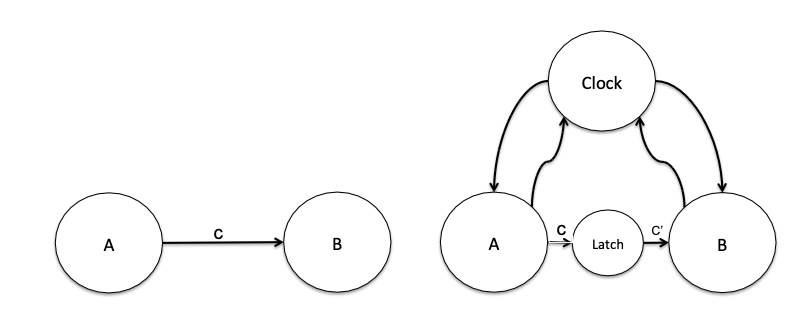
\includegraphics[width=0.7\linewidth]{Pictures/CSP.png}
  \caption{Enforcing global synchrony on a simple CSP model, where the channel \textbf{C} transfer information from the process \textbf{A} to process \textbf{B}, resulting in an increasing complexity. Figure from [\cite{vinter2014synchronous}]}
  \label{fig:csp}
\end{figure}

\section{Synchronous Message Exchange}
\label{sec:SME}

Most of this theory is based on [\cite{vinter2014synchronous}] and [\cite{SME2020}].
The motivation behind SMEs rose from the need to provide a simple framework for programming an FPGA.
It is an environment for developing and testing hardware designs for FPGAs in C\#. With SME, it is possible to create hardware structures translated to VHDL. 
However, FPGAs can be a better choice for energy-sensitive applications since FPGAs can, in some cases, achieve the same performance as a GPU but with lower energy consumption [\cite{SME2020}].
Previously, the developer needed to design an integrated circuit on the gate level for the FPGA. This could be difficult due to the low-level languages' design framework, which is not common knowledge amongst software developers. Some high-level methods for programming an FPGA have been developed. However, these are often tedious to work with. Thus, designing and implementing hardware models is beneficial with SME.\\

The goal with SME is to give software developers a tool that provides the opportunity to program hardware but with an added abstraction layer that separates the developer from the hardware details. The development resembles the structures and semantics known from software development.


The idea is to develop individual processes, test them through simulations and then connect them to larger hardware models. Leveraging the features of a modern $C\#$ Integrated Development Environment, such as Visual Studio, makes it much faster to develop, experiment, and test FPGA designs, especially for a software developer. SMEs add a software abstraction layer that conceals the complexity typically requiring high-level FPGA expertise.
SME was built on the requirements of a
\textbf{Hidden clock }, 
\textbf{Global synchronization}, 
\textbf{Broadcasting channels (Busses)}, 
\textbf{Shared nothing } and 
\textbf{Implicit latches }.\\


\subsection{The hidden clock and global synchronization}
Many factors have to be considered when writing in hardware, such as timing. Since processes could read and write signals, there is no way of knowing if the following processes would use old or new data. Therefore, some predictability for the hardware is required, so global synchronization is needed.
The hidden clock is made to establish coordination between processes by synchronizing them all. An SME model consists of clock cycles and one hidden clock that is then propagated out to all the processes having a clock cycle and activates them.
A clock cycle is a period between each signal, divided by all processes.
An SME clock cycle consists of three phases: reading, computing, and writing. The visual explanation could be shown as a step function going from high to low, see Figure \ref{fig:clock}, The process is activated on the rising clock when the process is executed where it reads from the bus, and then it computes and writes to the bus, all in one clock
cycle. Just before the rising edge of the clock, all signals are propagated on all busses, which means that all communication happens simultaneously.
Un-clocked processes will first be activated when the input has been written to by other methods processes.

\begin{figure}
  \centering
  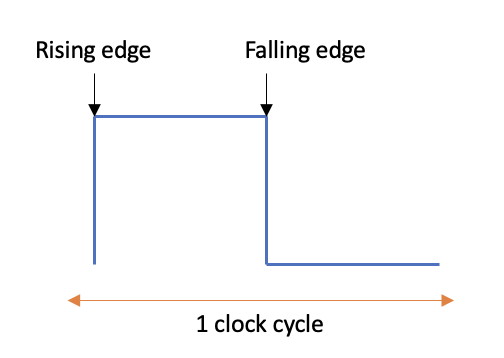
\includegraphics[width=0.5\linewidth]{Pictures/clockcycle.png}
  \caption{Illustration of a clock cycle}
  \label{fig:clock}
\end{figure}

The SME model supports both synchronous and asynchronous processes, whereby synchronous processes run during every clock cycle. In contrast, an asynchronous process is only run when receiving all of the signals on its input buses. 



\subsection{Broadcasting and busses}
In CSP, processes communicate with each other using channels that use the rendezvous protocol, meaning that data gets transmitted through the channel once the destination says it is ready to receive and vice versa.
On the contrary, SMEs use broadcasting channels called busses, from which any process can be read. This means that a process can broadcast its output to multiple processes through a single bus. Using CSP, multiple channels would have to emulate a single bus in SME. The busses define and manage the data that is exchanged between processes. These can be visualized as a pipe or a channel. When data is written to a bus it
will be available in the following clock cycle if it is a clocked process and available right
away for un-clocked processes. Furthermore, a bus can contain multiple data types and values that a process can access. 

\begin{figure}[H]
  \centering
  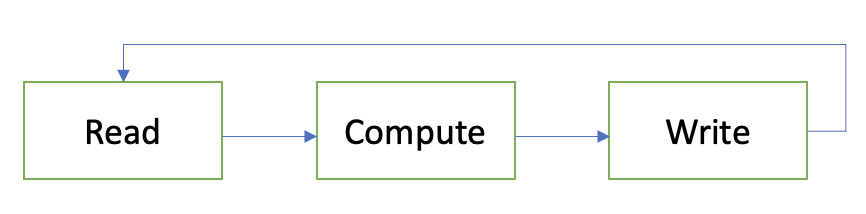
\includegraphics[width=0.7\linewidth]{Pictures/readbus.png}
  \caption{SME process for one clock cycle.}
  \label{fig:readbus}
\end{figure}


\subsection{Shared nothing}
The fastest way to handle data through hardware is by addressing memory separately.
A \acrshort{SN} is a distributed computing architecture in which you have several separate nodes that do not share memory or storage.
Operating under numerous self-sufficient nodes rather than having a single source of particular resources offers several advantages: easier scaling, non-disruptive upgrades, eliminating a single point of failure, and self-healing capabilities.
SN eliminates single points of failure, allowing the overall system to continue operating despite losses in individual nodes and allowing individual nodes to upgrade without a system-wide shutdown [\cite{sharednothing}]. 

\newpage


\section{Hardware Description Language}
Generally, implementing code down to \acrshort{FPGA} is programmed using Very High-Speed Integrated Circuit HDL \acrshort{VHDL}. This is harder to use since it is intended primarily to be a parallel programming language. This can be challenging, especially for a software engineer implementing an FPGA.
The vendors are not implementing recent updates to VHDL, and so it is not evolving with time or the programmer [\cite{SME2020}]. \\

The SME framework is implemented in the .NET framework, the version of SME that will be used throughout this thesis.
With the C\# SME library, it is possible to write all control logic in C\#.
All data written to a bus can be logged for each clock cycle and saved as a test bench, a piece of software used for
testing hardware models. It provides input data to the hardware model and verifies its output which is saved as a \acrshort{CSV}. Hence, it can then be used for compiling the program into VHDL, which can be put onto FPGA circuits. This eliminates the need to write a separate VHDL test bench, which immensely improves developer productivity. This is needed since some of the implementations are still manually done to implement on hardware, which will be in Vivado. A further explanation of the performance can be found in Chapter~\ref{cha:implementation}.




\section{SME setup and structure}

To show the basic structure of how SMEs works, we will go over the fundamental design. For further explanation on how the system was set up for the whole project, see Chapter \ref{cha:implementation}.
When analyzing the general structure of our SME program, there are three main structures:
\begin{enumerate}
    \item \textbf{Connection}: How the circuit is connected, i.e., which busses connect to which processes.
    \item \textbf{Processes}: The process structure for each function and how they behave.
    \item \textbf{Verification data}: All data from the Python FNN that could be useful for the verification of the hardware model.
\end{enumerate}



\subsection{Connection}

The fundamental structure behind the SME network is the communication between the processes through busses. Understanding different communication structures in SMEs will provide the insight necessary for designing the translated systems of the Python model.
A network in an SME program is a crucial part that connects all processes with
communication. Defining the network from process instances
also has the advantage that one process can be instantiated with different parameters several
times within the same network, providing the possibility of reusing the processes for different
purposes.

\subsubsection{Busses}
As previously explained, an SME bus defines a collection of channels used for all
communication between the processes. Each channel has a type describing the communicated
data and can be initialized with an initial value. The IBus interface marks an interface as a bus of a read or writes in SME, which is shown as an example in Listing \ref{lst:bus} where we define a \emph{bus} to transfer a value. 
An SME bus has an identifier used for referencing the bus. All channels within a bus are connected to the process simultaneously, and it is up to the developer to call the correct channel within the bus for either a read or a write. 

\begin{listing}
  \inputminted{csharp}{codesnippets/bus_value.cs}
  \caption{Simple bus that transfers one value}
  \label{lst:bus}
\end{listing}


\iffalse
\begin{listing}
  \inputminted{csharp}{codesnippets/bus_example.cs}
  \caption{bus that transfers an index and is set to with a Boolean}
  \label{lst:bus_example}
\end{listing}
\fi

\subsection{Process structure}
The processes in an SME program describe the fundamental behavior of a model.
An SME process is defined by the \emph{SimpleProcess} class and consists of an identifier, process parameters, bus, and variable declarations. The body of the process, the process statements, consists
of sequential notices such as communications and calculations to be evaluated once
for each clock cycle. 
%A small example of an SME process has been presented in Appendix \ref{appendix:Sme_guide}.

A process is initiated in the network of an SME program. A process can be instantiated with a set of parameters. These parameters can
be a mix of input and output busses and constants.

When defining a process, we can give either an \textbf{Input Bus} or a \textbf{Output Bus}.
The name of the input bus can be given as a process parameter, which the process can use to read from the actual bus channel, as can be seen in App. \ref{appendix:Sme_guide} Listing \ref{lst:sigmoidSME}. In this example, the process reads the data from \emph{m\_input} in the bus and writes the data to the \emph{m\_output}.




\subsection{Verification data}
It will always be necessary to generate input for pure SME networks, which can be done in multiple ways. One way of initializing the SME network data is by giving the process a constant given as a parameter or by hard-coding internal values into the process. Another way is to have a separate process that generates data for the network. The first attempt to write a process to generate data is shown in the example App. \ref{appendix:Sme_guide} Listing \ref{lst:sigsimulator}.
Here the process clock is a data generating process. It does not read data from any input bus. Thus, it can only create data to write to the network. The example shows the \texttt{Sigsimulator} which generates values from $[1,10]$ and writes it out onto the output bus. A further explanation of the structure of a process will be introduced further in Chapter \ref{cha:implementation}.
Another way to generate data is to make a process that imports the data and reads them through a bus. This was created as a simple SME process structure, where the function reads the data from a CSV file and saves it as a flat array. This is shown in Listing \ref{lst:datagenerator}.

An SME process that does not read any input is just a data generation process, but in this case, we use the input bus \emph{index} to make sure that each value that reads from the CSV file gets an index.
The output-bus transfers the array of data and makes sure it gets written out.
In \ref{lst:datagenerator} the \emph{async process} only runs when the index is ready.  The address will save each value and write them out in an array.


\begin{listing}
  \inputminted{csharp}{codesnippets/datagenerator.cs}
  \caption{C\# code to import an \emph{input} CSV file, using SME processes to save the data \emph{output} as a flat array}
  \label{lst:datagenerator}
\end{listing}

\newpage


\section{Related work}
As mentioned in Chapter \ref{cha:introduction}, FPGAs contain many exciting properties, which makes them more flexible to use, faster, and more energy-efficient than GPU/CPUs for specific tasks. Algorithms are getting more complex and energy-consuming.
FPGAs are not widespread due to the low-level language used to program the chip [\cite{fang2020memory}]. This has started a minor movement in building alternative implementation frames such as SME.
An exciting framework constructed from the same idea is \textbf{hls4ml}, which was made as a joint project between Xilinx and CERN for accelerating the inference of processing data [\cite{hls4ml}]. A growing team of physicists and engineers from CERN wanted to have a flexible way to optimize custom event filters in the Compact Muon Solenoid (CMS) detector they are working with at CERN. The very high data rates in the CMS detector required event processing in real-time, but trigger filter algorithm development hindered the team’s ability to make progress [\cite{fahim2021hls4ml}].
hls4ml is built on the idea of being a user-friendly software based on High-Level Synthesis (HLS), designed to deploy network architectures on FPGAs. This is done in $C$ as a sequential programming model designed for CPUs rather than FPGAs. As such, it is not uncomplicated to gain performance, as it relies on automatic derivation of parallelism.
Among others to describe hardware using higher-level language are \textbf{Chisel-lang} [\cite{chisel-lang}], which is similar to SME but described as a library in Scala. This means that the programmer needs to be able to keep two states of the program in mind, one that is running in Scala, evaluating some specific condition statements, and another running the generated code, not being able to see the condition statements [\cite{SME2020}].
\textbf{OpenCL }is a popular framework that intent to get more GPU programmers on board.[\cite{OpenCL}]
However, the focus here is not to accelerate with FPGAs, and as introduced in chapter \ref{cha:introduction}, the different hardware has different benefits.
And \textbf{QuokkaEvaluation} [\cite{QuokkaEvaluation}] is still an ongoing project focusing on specific FPGA implementations and has similar elements from SME, but is still in the initial phase.

